\documentclass{article}
\usepackage[a4paper, total={6.5in, 10in}]{geometry}
\setlength{\parindent}{0pt}
\usepackage[british]{babel}
\usepackage{amsfonts}
\usepackage{amssymb}
\usepackage{amsmath}
\usepackage{amsthm}
\usepackage{mathtools}
\usepackage{datetime2}
\usepackage{template/cenvs}
\usepackage{tikz}

\title{\textbf{Homework 2}}
\author{Robert O'Connell}
\date{\today}

\begin{document}
\maketitle

\begin{problem}
Suppose that \( x,y \) are distinct points in a metric space \( (X,d) \) and let \( \epsilon = \frac{d(x,y)}{2} \)

Prove that \( B_{\epsilon}(x) \) and \( B_{\epsilon}(y) \) are disjoint
%
% \begin{solution}
% 	Assume \( \exists \ x_{0} \in B_{\epsilon}(x) \) and \( y_{0} \in B_{\epsilon}(y) \) such that \( x_{0} = y_{0} \)
%
% 	Thus \( d(x_{0},x) = d(y_{0},y), d(x_{0},y), d(y_{0},x) \text{ are all } < \frac{d(x,y)}{2} \) and \( d(x_{0},y_{0}) = 0 \)
% 	Thus \( d(x_{0},x) = d(y_{0},x) \) and \( d(y_{0},y) = d(x_{0},y) \) are both \( < \frac{d(x,y)}{2} \)
%
% 	Then using the triangle inequality
% 	\begin{align*}
% 		d(y_{0},x) + d(y,y_{0}) \le d(x_{0},y_{0}) + d(x_{0},x) & + d(y_{0},y)                                       \\
% 		\frac{d(x,y)}{2} + \frac{d(x,y)}{2} \le d(x_{0},x)      & + d(y_{0},y) < \frac{d(x,y)}{2} + \frac{d(x,y)}{2}
% 	\end{align*}
% 	No such number \( d(x_{0},x) + d(y_{0},y) \) exists, a contradiction
% \end{solution}
\begin{solution}
	Assume there exists \( v \in B_{\epsilon}(x) \cap B_{\epsilon}(y) \)

	Then \( d(x,z) < \frac{d(x,y)}{2} \) and \( d(y,z) < \frac{d(x,y)}{2} \)

	\begin{align*}
		d(x,z) + d(y,z)            & < d(x,y) \\
		d(x,y) \le d(x,z) + d(z,y) & < d(x,y) \\
		d(x,y)                     & < d(x,y)
	\end{align*}

	A contradiction, hence the intersection of the two balls is empty, meaning they are disjoint
\end{solution}
\end{problem}

\begin{problem}
Sketch the open ball \( B_1^{d_{\infty}}((0,0)) \) in \( \mathbb{R}^2 \)

\begin{solution}
	\begin{center}
		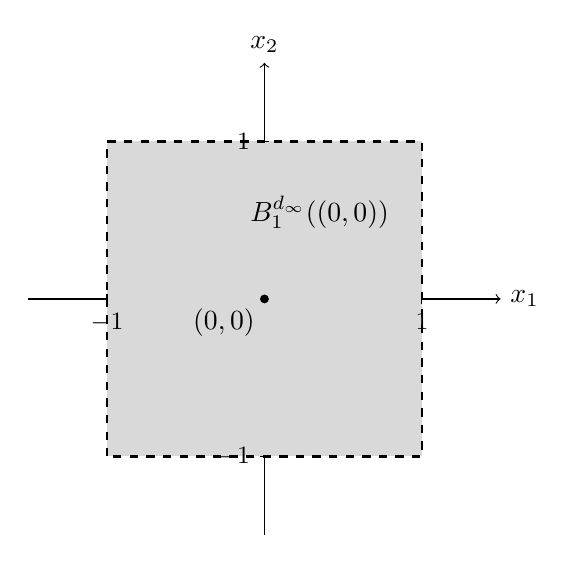
\begin{tikzpicture}[scale=2]
			% axes
			\draw[->] (-1.5,0) -- (1.5,0) node[right] {$x_1$};
			\draw[->] (0,-1.5) -- (0,1.5) node[above] {$x_2$};

			% open square (interior shaded, boundary dashed)
			\fill[gray!30] (-1,-1) rectangle (1,1);
			\draw[dashed, thick] (-1,-1) rectangle (1,1);

			% center
			\fill (0,0) circle (0.8pt) node[below left] {$(0,0)$};

			% tick labels
			\foreach \x in {-1,1} {
					\draw (\x,0.03) -- (\x,-0.03) node[below] {\small $\x$};
					\draw (0.03,\x) -- (-0.03,\x) node[left] {\small $\x$};
				}

			% label
			\node at (0.35,0.55) {$B_1^{d_\infty}((0,0))$};
		\end{tikzpicture}
	\end{center}
\end{solution}
\end{problem}

\begin{problem}
Prove that a subset of a metric space is open iff it is a union of open balls

\begin{solution}
	Let \( (X,d) \) be a metric space and \( U \subset X \)

	(\( \Rightarrow \))

	Assume \( U \) is open

	Then \( \forall \ x \in U \ \exists \ \epsilon_x > 0  \) s.t. \( B_{\epsilon_x} \subset U \)

	Then looking at \( \cup_{x \in U} B_{\epsilon_x}(x) \)

	If \( u \in U \), then certainly \( u \in B_{\epsilon_u}(u) \), so \( u \in \cup_{x \in U}B_{\epsilon_x}(x) \)

	If \( u \in \cup_{x \in U} B_{\epsilon_x}(x) \), then \( u \in B_{\epsilon_x}(x) \) for some \( x \), which is a subset of \( U \), so \( u \in U \)

	Thus \( U = \cup_{x \in U}B_{\epsilon_x}(x) \)
	\\

	(\( \Leftarrow \))

	\begin{lemma}
		Let \( (X,d) \) be a metric space

		Any open ball is an open set

		\begin{proof}
			Let \( \epsilon > 0  \) and \( x_0 \in X \) and consider \( B_{\epsilon}(x_{0}) \subset X \)

			Let \( x \in B_{\epsilon}(x_{0}) \), choose \( \epsilon_x = \epsilon - d(x,x_{0}) \)

			Consider \( B_{\epsilon_x}(x) \)

			If \( y \in B_{\epsilon_x}(x) \) then \( d(x,y) < \epsilon_x = \epsilon - d(x,x_{0}) \)

			\( \Rightarrow d(y,x) + d(x,x_{0}) < \epsilon \Rightarrow d(y,x_{0}) < \epsilon \) by the triangle inequality.

			Thus \( y \in B_{\epsilon}(x_{0}) \) and then \( B_{{\epsilon_x}}(x) \subset B_{\epsilon}(x_{0}) \)

			Thus \( B_{\epsilon}(x_{0}) \) is an open set
		\end{proof}
	\end{lemma}

	Let \( \cup_{a \in A} B_{\epsilon_a}(a) \) be a union of open balls in \( X \)

	From the above lemma \( \cup _{a \in A}B_{\epsilon_a}(a) \) is also a union of open sets.

	Then from lecture the union of opens sets is also open, so \( \cup _{a \in A} B_{\epsilon_a}(a) \) is an open set

\end{solution}
\end{problem}

\begin{problem}
Suppose that in a metric space \( X \) we have \( B_r(x) = B_s(y) \) for some \( x,y \in X \) and some positive real numbers \( r,s \)

Is \( x= y \)? and is \( r=s \)?

\begin{solution}
	It is not true in general that \( x=y \) and \( r=s \)

	Consider the metric space of \( (\mathbb{R}^n, d) \) for any \( n \), where \( d(x,y) = \begin{cases}
		0 \text{ if } x=y \\
		1 \text{ if } x \neq y
	\end{cases} \)

	Now for any \( r > 1 \) we have that \( B_r(x) = \mathbb{R}^n \) for all \( x \in \mathbb{R}^n \)

	For \( n=1 \), we can take \( x = 1 \) and \( y =  2 \), \( r = 2 \) and \( s = 3 \), we have \( B_r(x) = B_s(y) = \mathbb{R} \) while \( x \neq y \) and \( r \neq s \)
\end{solution}
\end{problem}

\begin{problem}
Which of the following sets are closed in \( \mathbb{R} \)?
\begin{itemize}
	\item \( [1,\infty) \)
	\item \( \mathbb{R} \setminus \mathbb{Q} \)
	\item \( \left\{ \frac{n}{n+1} \mid n \in \mathbb{N} \right\}  \)
	\item \( \left\{ \frac{1}{n} \mid n \in \mathbb{N}, n \ge 2 \right\} \cup \left\{ 0,1,2 \right\}  \)
\end{itemize}

\begin{solution}1.

	To check whether \( [1,\infty) \) is closed, we need to see whether \( \mathbb{R}\setminus [1,\infty) = (-\infty,1) \) is open.


	For \( (-\infty,1) \) to be open, we need \( B_{\epsilon}(x) \subset (-\infty,1) \) for all \( x \in (-\infty,1) \)

	Let \( x \in (-\infty,1) \), choose \( \epsilon = \frac{|x-1|}{2} \)

	If \( y \in B_{\epsilon}(x) \), then \( |x-y| < \epsilon = \frac{|x-1|}{2} \)

	So,
	\begin{align*}
		-\frac{|x-1|}{2} < x- & y                       \\
		                      & y < \frac{|x-1|}{2} + x
	\end{align*}

	Since \( x \in (-\infty,1) \Rightarrow x-1 \le 0 \Rightarrow |x-1| = 1 - x\)

	Then \( y < x - \frac{x-1}{2} = \frac{1}{2}(x + 1) \)

	Let \( f \colon \R \to \R \colon f(x) = \frac{1}{2}(x+1)  \)

	Clearly \( f \) is increasing since \( f' > 0 \)

	Thus \( \forall \ x \in (-\infty,1) \) \( f(x) < f(1) = 1 \)

	So \( y < 1 \) so \( B_{\epsilon}(x) \subset (-\infty,1)\)

	Hence \( (-\infty,1) \) is open, so \( [1,\infty) \) is closed
\end{solution}

\begin{solution} 2.

	\begin{lemma}
		Between any two rational numbers \( a, b \), \( a < b \) there exists an irrational number

		\begin{proof}
			Let \( r = a + \frac{b-a}{\sqrt{2} } \)

			Clearly \( \frac{b-a}{\sqrt{2}} > 0 \) so \( a < r \), and also \( b-a > r-a = \frac{b-a}{\sqrt{2} } \)

			Combining these we get \( a < r < b \)
			\\

			Assume \( r \) is rational and can therefore be written as the ratio of two coprime integers \( p,q, q \neq 0 \)
			\[
				r = a + \frac{b-a}{\sqrt{2} }
			\]
			\[
				\Rightarrow \sqrt{2}  = \frac{b-a}{r - a}
			\]
			Since \( r \neq a \) we have \( \sqrt{2}  \) as the ratio of rationals, since the sums of rationals are rationals, which is rational

			A contradiction to the fact that \( \sqrt{2}  \) is known to be irrational

			Hence \( r \) is irrational
		\end{proof}
	\end{lemma}

	Assume for the sake of contradiction that \( \mathbb{R}\setminus \mathbb{Q} \) is closed then \( \mathbb{R} \setminus (\mathbb{R} \setminus \mathbb{Q} ) = \mathbb{Q} \) is open

	But we know that \( \mathbb{Q} \) is not open

	Let \( q \in \mathbb{Q} \) and \( \epsilon > 0 \)
	\[
		B_{\epsilon}(q) = \left\{ x \in \mathbb{R} \mid |x-q| < \epsilon \right\}
	\]
	We can find two rationals in \( B_{\epsilon}(q) \), for example \( q \pm \frac{\epsilon}{2} \), then from the above lemma there exists some \( r \in \mathbb{R}\setminus \mathbb{Q} \) such that \( r \in B_{\epsilon}(q) \)

	Hence \( B_{\epsilon}(q) \not\subset \mathbb{Q}\)

	Hence \( \mathbb{Q} \) is not open

	Hence \( \mathbb{R} \setminus \mathbb{Q} \) is not closed
\end{solution}


\begin{solution} 3.

	If \( A = \left\{ 1 - \frac{1}{n+1} \mid n \in \mathbb{N} \right\}  \) is closed than \( \overline{A} = A \)

	Clearly \( 1 \notin A \) since \( \frac{1}{n+1} \neq 0 \) for all \( n \in \mathbb{N} \)

	But we can create a sequence \( x_n \) with \( x_n \in A \) for all \( n \in \mathbb{N} \), which converges to 1, \( \left\{ x_n = 1 - \frac{1}{n+1} | n \in \mathbb{N} \right\}  \). This obviously converges to 1, since \( \frac{1}{n+1} \to 0 \). Thus from the sequential characterization of the closure \( 1 \in \overline{A} \)

	Since \( 1 \notin A \) and \( 1 \in \overline{A} \) this implies \( \overline{A} \neq A \), and hence \( A \) is not closed

\end{solution}

\begin{solution} 4.

	First we will find the limit points of \( A = \left\{ \frac{1}{n} \mid n \in \mathbb{N} \right\} \cup \left\{ 0,1,2 \right\}  \)

	It is clear from the definition of a limit point that the right hand side of the union has no limit points, since for \( \epsilon = \frac{1}{2} \) \( B_{\epsilon}(x)\setminus \left\{ x \right\}  \cap \{0,1,2\} = \emptyset \) for all \( x \in \left\{ 0,1,2 \right\}  \)

	We can also see that \( 0 \) is a limit point of the left hand side, consider the sequence \( \left\{ x_n = \frac{1}{n} \right\}_{n=2}^{\infty}  \), this is clearly convergent to \( 0 \) and with each of the \( x_n \in A \) and \( x_n \neq 0 \) for all \( n \in \mathbb{N} \)

	Consider any \( a < 0 \), every element of \( A \) is greater or equal to zero, so \( B_{\frac{|a|}{2}}(a) = \left( \frac{3a}{2}, \frac{a}{2} \right)  \) does not intersect with \( A \), so no \( a < 0 \) is a limit point

	Now consider any \( a > 0 \). \( B_{\frac{a}{2}}(a) = \left( \frac{a}{2}, \frac{3a}{2} \right)  \), a point \( \frac{1}{n} \in A, n \in \mathbb{N} \) lies in the ball iff \( \frac{1}{n} > \frac{a}{2} \Rightarrow n < \frac{2}{a} \). Only a finite number of \( n \) can satisfy this, hence the ball contains a finite amount of elements in \( A \). Let \( \epsilon \) be the minimum of all of the distances between the points of \( a \) in \( B_{\frac{a}{2}}(a) \setminus \left\{ a \right\}  \) to \( a \). By construction, \( B_{\epsilon}(a) \setminus \left\{ a \right\}  \cap A = \emptyset \), so no \( a > 0 \) is a limit point.

	Hence \( 0 \) is the only limit point of \( A \)

	But \( 0 \in A \), so \( \overline{A} = A \cup A' = A  \), hence \( A \) is closed

\end{solution}
%
% \begin{solution} 3.
%
% 	If \( A = \left\{ 1 - \frac{1}{n+1} \mid n \in \mathbb{N} \right\} \) is closed, that means its complement with respect to \( \mathbb{R} \), \( \mathbb{R} \setminus A \) is open
%
% 	Let \( \epsilon > 0  \) and consider the ball \( B_{\epsilon}(1) \)
% 	\[
% 		B_{\epsilon}(1) = \left\{ x \in \mathbb{R} \mid |x-1| < \epsilon \right\}
% 	\]
%
% 	% for any \( \epsilon > 0 \) we see that \( B_{\epsilon}(1) \cup A \neq \emptyset \)
%
% 	% Clearly \( 1 \in \mathbb{R} \setminus A \), since \( 0 \) is not attained by the function \( \frac{1}{n+1} \) meaning \( 1 \notin A \)
% 	Since \( 0 \) is not attained by \( \frac{1}{n+1} \) for all \( n \in \mathbb{N} \), \( \Rightarrow 1 \notin A \Rightarrow 1 \in \mathbb{R} \setminus A \)
%
% 	Then choose \( x \in \mathbb{N} \) such that \( 1 - \frac{1}{x+1} < \epsilon \)
%
% 	Then \( 1 - \frac{1}{x+1} \in B_{\epsilon}(1)  \) but also \( 1 - \frac{1}{x+1} \in A \), hence \( B_{\epsilon}(1) \cap A \neq \emptyset \)
%
% 	So \( B_{\epsilon}(1) \not\subset \mathbb{R} \setminus A \), so the complement of \( A \) is not open, so \( A \) is not closed
% \end{solution}
%











% \begin{solution} 3.
%
% 	\begin{lemma}
% 		Let \( (X,d) \) be a metric space
%
% 		A set \( A \subset X \) with \( A \) containing a single element \( x \) is closed
%
% 		\begin{proof}
% 			\( A \) closed if \( X\setminus A = X \setminus \left\{ x \right\} \) is open
%
% 			Let \( y \in X \setminus \left\{ x \right\}  \), choose \( \epsilon = \frac{d(x,y)}{2} \)
%
% 			Then \( B_{\epsilon}(y) \subset X \setminus \left\{ x \right\} \iff x \notin B_{\epsilon}(y) \)
%
% 			\( x \in B_{\epsilon}(y) \iff d(x,y) < \frac{d(x,y)}{2} \)
%
% 			Since \( 0 \le d(a,b), \quad \forall \ a,b \in X \) this is not true
%
% 			Hence \( x \notin B_{\epsilon}(y) \), so \( B_{\epsilon}(y) \subset X \setminus\left\{ x \right\} \)
%
% 			Thus \( X \setminus \left\{ x \right\}  \) is open and so \( A \) is closed
% 		\end{proof}
% 	\end{lemma}
%
% 	We can write \( \left\{ \frac{n}{n+1} \mid n \in \mathbb{N} \right\}  \) as \( \cup _{n \in \mathbb{N}}{\frac{n}{n+1}} \), which is as the union of sets containing a single element
%
% 	Which from the lemma above are all closed. Then from lecture we have that the union of closed sets is closed
% \end{solution}
%






%
% \begin{solution} 3.
%
% 	Assume for the sake of contradiction that \( \left\{ \frac{n}{n+1} = 1 - \frac{1}{n} \mid n \in \mathbb{N} \right\}  \) is closed
%
% 	Then its complement \( A = \left\{ (-\infty,0) \cup [1,\infty) \right\}  \) must be open
%
% 	Let \( x = 1 \) and \( \epsilon>0 \)
%
% 	Clearly \( 1-\frac{\epsilon}{2} \in B_{\epsilon}(1) \) but also \( 1- \frac{\epsilon}{2} \notin A \)
%
% 	Hence \( B_{\epsilon}(1) \not\subset A \)
%
% 	A contradiction to the fact that \( A \) is open
%
% 	Hence \( \left\{ \frac{n}{n+1} \mid n \in \mathbb{N} \right\}  \) is not closed
%
% \end{solution}
%
% \begin{solution} 4.
%
% 	\[
% 		\left\{ \frac{1}{n} \mid n \in N, n \ge 2 \right\} \cup \{0,1,2\} = (0,1 / 2] \cup \{0,1,2\} = [0,1 / 2] \cup \{1,2\}
% 	\]
% 	From lecture we have that the union of finetly many closed sets is closed, so it suffices to prove each of the sets seperately
%
% 	The complement of \( [0, 1 /2]\) is \( A = (-\infty,0) \cup (1 /2, \infty) \)
%
% 	Let \( x \in A \) and choose \( \epsilon = \begin{cases}
% 		\frac{x}{2} \text{ if } x < 0 \\
% 		\frac{x - \frac{1}{2}}{2} \text{ if } x > \frac{1}{2}
% 	\end{cases} \)
%
% 	Then if \( x < 0 \), \( y \in B_{\epsilon}(x) = \left\{ a \in \mathbb{R} \mid |x-a| < \frac{x}{2} \right\} \Rightarrow y < \frac{3x}{2} < 0 \) so \( B_{\epsilon}(x) \subset A \)
%
% 	If \( x > \frac{1}{2} \), \( y \in  B_{\epsilon}(x) = \left\{ a \in \mathbb{R} \mid |x-a| < \frac{x}{2} - \frac{1}{4} \right\} \Rightarrow \frac{1}{2} \le \frac{x}{2} + \frac{1}{4} < y  \) so \( B_{\epsilon}(x) \subset A \)
%
% 	Thus \( A \) is open, hence \( [0, 1 /2] \) is closed
% 	\\
%
% 	The complement of \( \left\{ 1, 2 \right\}  \) is \( A = \mathbb{R} \setminus \left\{ 1,2 \right\}  \)
%
% 	Let \( x \in A \) and choose \( \epsilon = \begin{cases}
% 		1- x \text{ if } x < 1                                         \\
% 		\frac{\min\left\{ x-1, 2-x \right\} }{2} \text{ if } 1 < x < 2 \\
% 		x - 2 \text{ if } x > 2
% 	\end{cases} \)
%
% 	If \( x < 1 \), \( y \in B_{\epsilon}(x) = \left\{ a \in \mathbb{R} \mid |x-a| < 1 -x \right\} \Rightarrow y < 1 \) so \( B_{\epsilon}(x) \subset A \)
%
% 	If \( 1 < x < 2 \), \( y \in B_{\epsilon}(x) = \left\{ a \in \mathbb{R} \mid |x-a| < \min\left\{ x-1, 2-x \right\}  \right\}  \)
%
% 	Case (i) \( \min \left\{ \ldots  \right\} = x-1   \),
%
% 	\( \Rightarrow - x + 1 <y -x < x-1 \Rightarrow 1 < y < 2x -1 \le 2 \) since \( x \le \frac{3}{2} \)
%
% 	Case (ii) \( \min \left\{ \ldots  \right\} = 2 -x  \),
%
% 	\( \Rightarrow x -2 < y - x < 2 -x \Rightarrow 1 < 2(x -1) < y < 2 \) since \( x > \frac{3}{2} \)
%
% 	In either of these cases \( y \in A \)
% 	\\
%
% 	If \( x > 2 \), \( Y \in B_{\epsilon}(x) = \left\{ a \in \mathbb{R} \mid |x-a| < x -2 \right\} \Rightarrow 2 < y  \), so \( B_{\epsilon}(x) \subset A \)
% 	\\
%
% 	In all of the above cases \( y \in B_{\epsilon}(x) \Rightarrow y \in A \), hence \( B_{\epsilon}(x) \subset A \)
%
% 	Hence \( A \) is open
%
% 	Hence \( \left\{ 1,2 \right\}  \) is closed
%
% 	Hence the union of the two sets is closed
% \end{solution}
\end{problem}

\end{document}

